\section{Тренировочное задание}

Вариант: 0.

Начало: 01.03.2021.

Конец: 07.04.2021.

Продолжительность: 28 дней.

\begin{figure}[H]
	\centering
	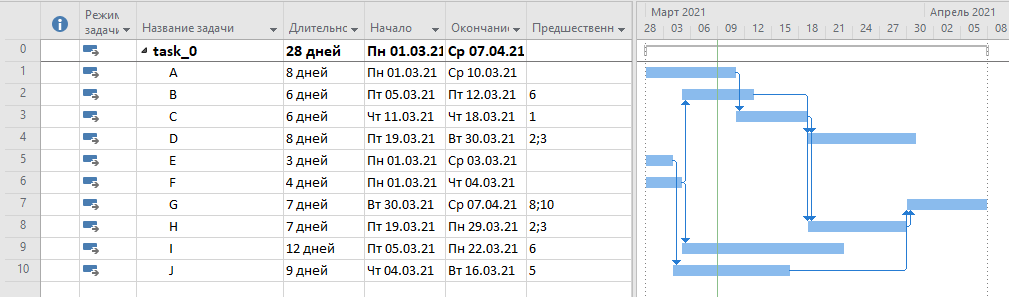
\includegraphics[width=0.8\textwidth]{img/content/task_0.png}
	\caption{Тренировочное задание}
\end{figure}

Рабочий день длился 8 часов, с 9 до 18. Тип задач -- фиксированный объем ресурсов.

\section{Условие}

Содержание проекта: Команда разработчиков из 16 человек занимается созданием карты города на основе собственного модуля отображения. Проект должен быть завершен в течение 6 месяцев. Бюджет проекта: 50 000 рублей.


\section{Задание 1}

Настройка рабочей среды проекта.

В настройках параметром, устанавливаем необходимое:

\begin{itemize}
	\item Дата начала проекта -- первый рабочий день марта текущего года.
	\item Длительность работы в неделях, объем работ в часах, а тип работ -- с фиксированными трудозатратами.
	\item Количество рабочих часов в день -- 8, количество рабочих часов в неделю -- 40.
	\item Начало рабочей недели в понедельник, а финансового года -- в январе.
	\item Продолжительность рабочего дня с 9 до 18 часов.
\end{itemize}

\begin{figure}[H]
	\centering
	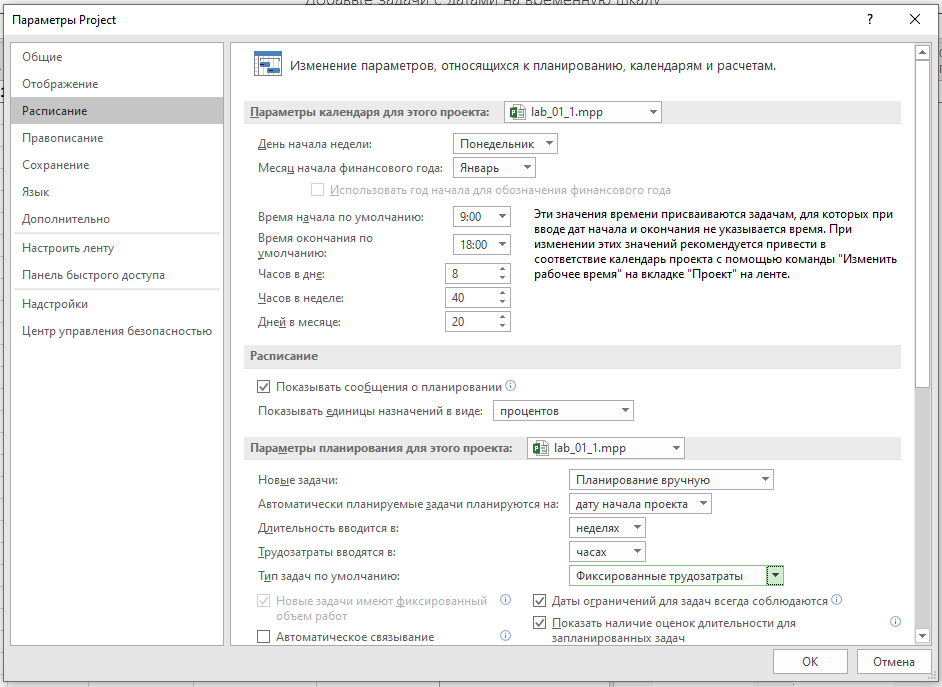
\includegraphics[width=0.8\textwidth]{img/content/settings.png}
	\caption{Настройка параметров}
\end{figure}

Дальше, были отмечены все выходные и праздничные дни на ближайшие календарные месяцы от даты начала проекта.

\begin{figure}[H]
	\centering
	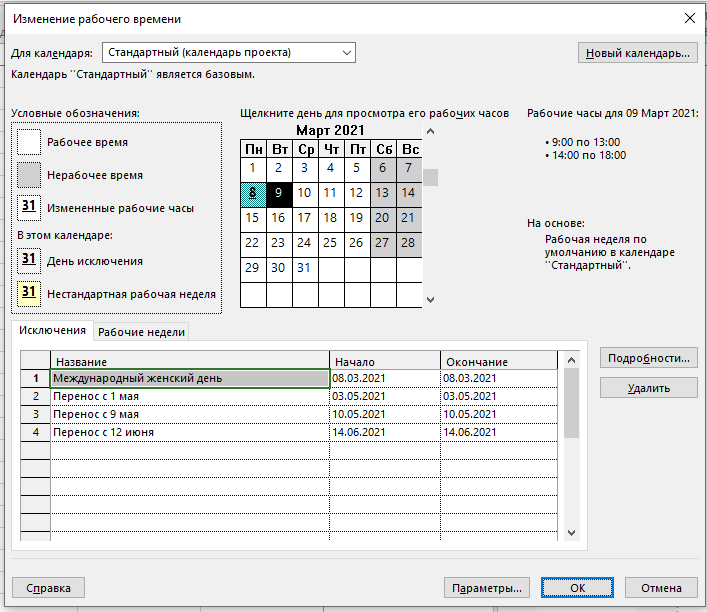
\includegraphics[width=0.8\textwidth]{img/content/calendar.png}
	\caption{Добавление выходных и праздников}
\end{figure}

Добавлена суммарная задача проекта и заметка с краткой информацией о нем.

\begin{figure}[H]
	\centering
	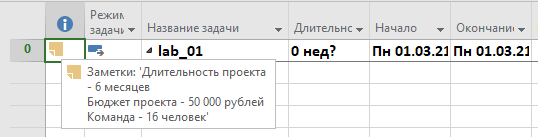
\includegraphics[width=0.8\textwidth]{img/content/summary.png}
	\caption{Суммарная задача с описанием}
\end{figure}

\section{Задание 2}

Вводим список задач, в соотвествии с заданной таблицей.

Задачи 1 и 27 являются задачами вехами, они обозначают начало или конец фазы проекта и имеют нулевую продолжительность.

Задачи 2, 3, 8, 12,19 и 22 будут преобразованы в фазы проекта, поэтому длительность для них не указываем.

\begin{figure}[H]
	\centering
	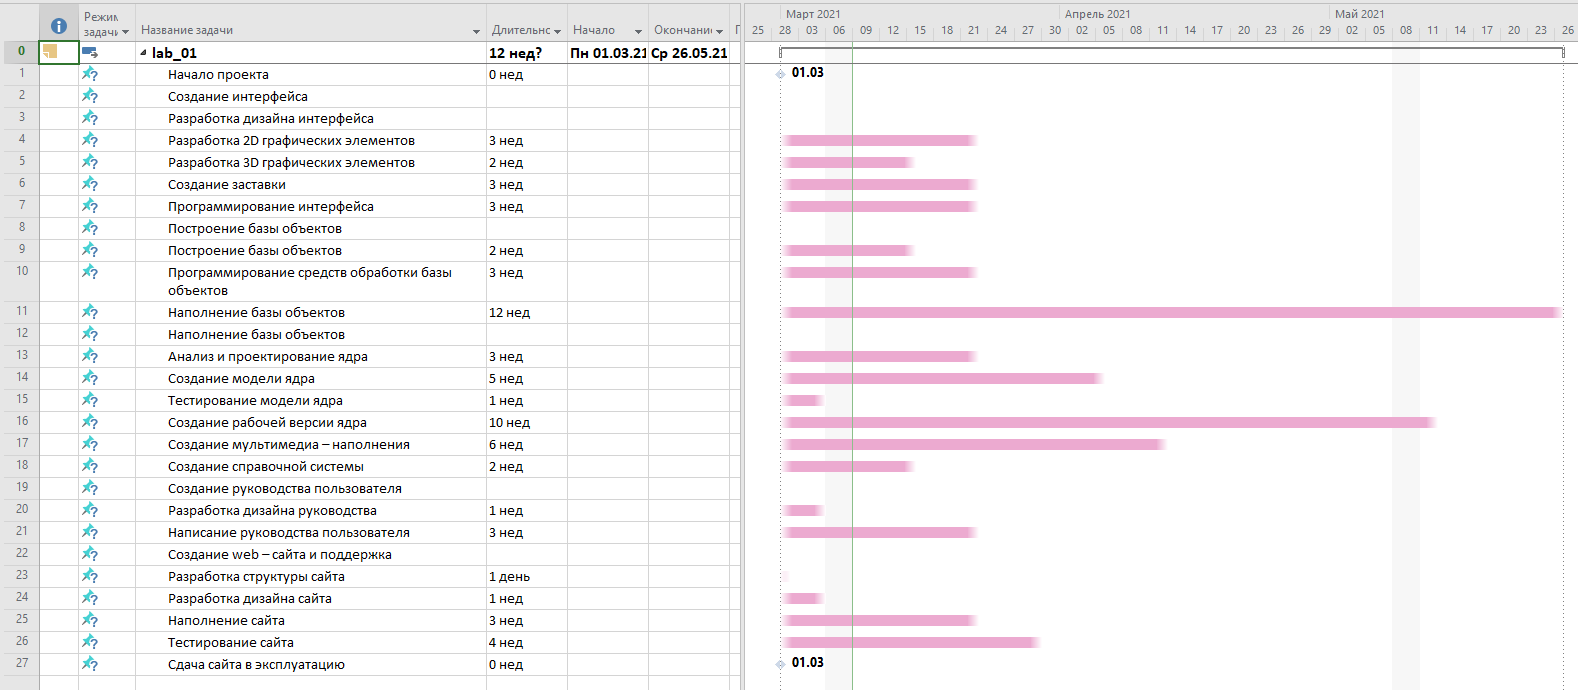
\includegraphics[width=0.8\textwidth]{img/content/tasks.png}
	\caption{Список задач}
\end{figure}

\section{Задание 3}

Дальше группируем задачи как подзадачи.

\begin{figure}[H]
	\centering
	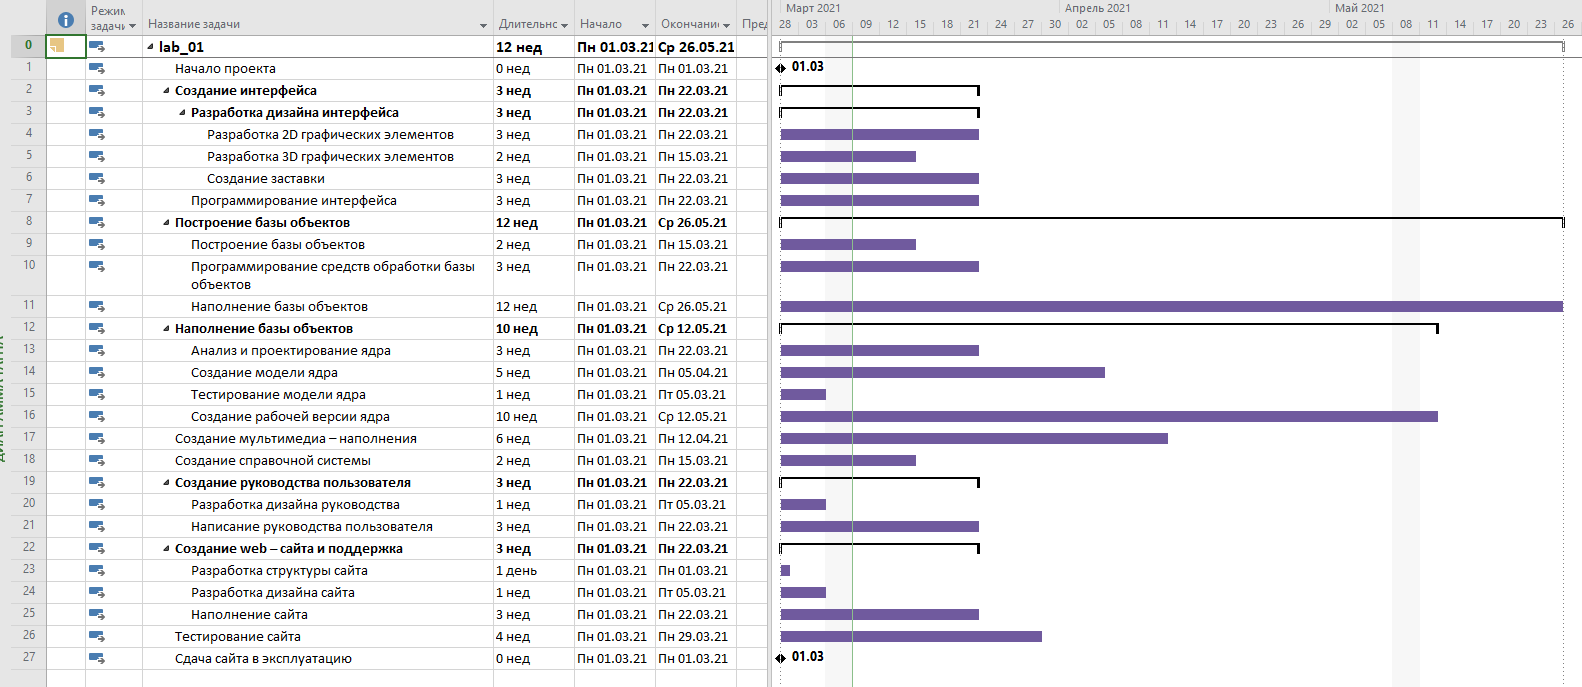
\includegraphics[width=0.8\textwidth]{img/content/struct_tasks.png}
	\caption{Структурирование списка задач}
\end{figure}

\section{Задание 4}

Далее связываем задачи между собой: НН -- задачи начинаются одновременно, ОН -- задача начинается после окончания предыдущей. Также можно ввести запаздывание -- положительное число и опережение -- отрицательное число.

\begin{figure}[H]
	\centering
	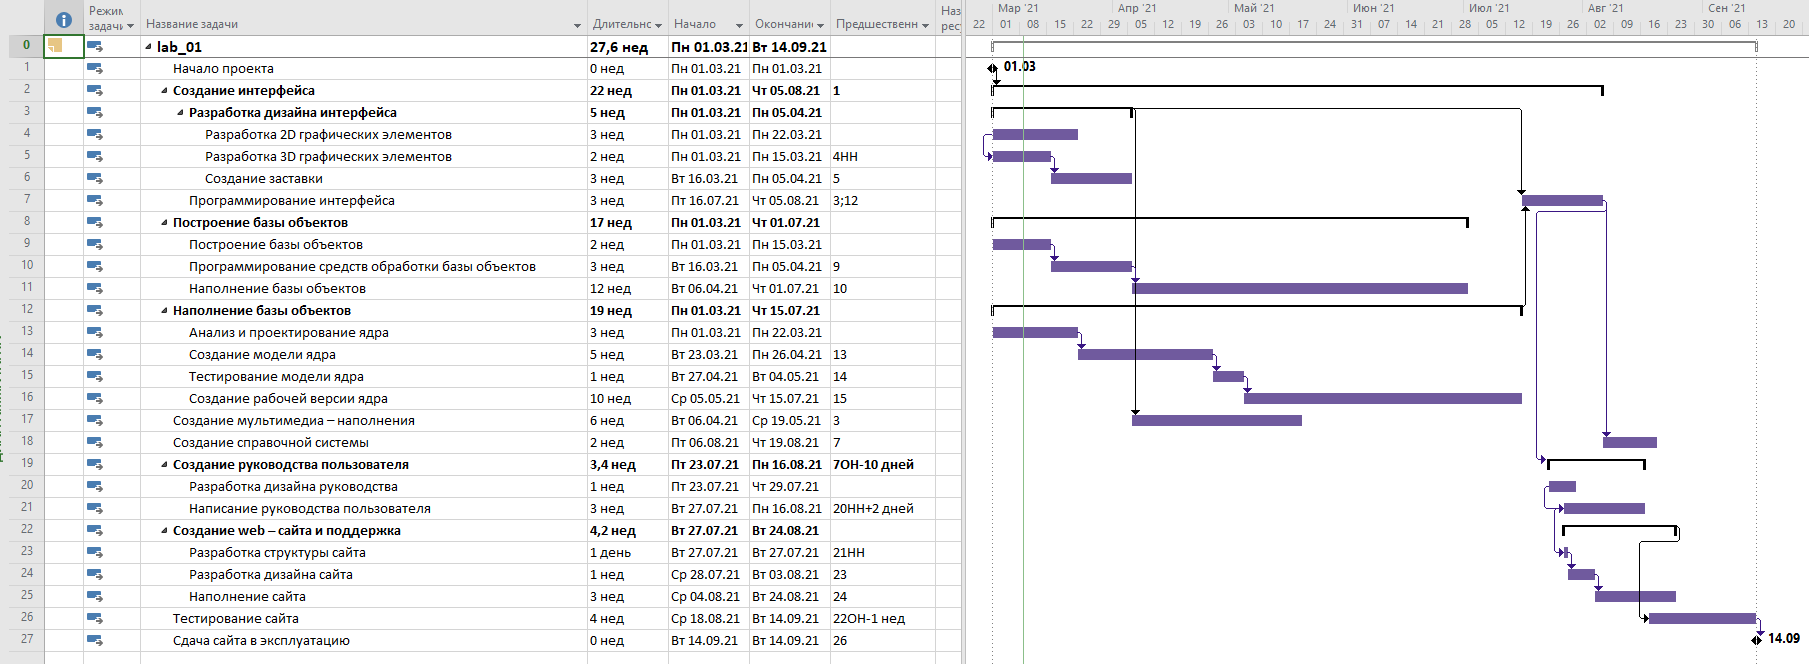
\includegraphics[width=0.8\textwidth]{img/content/link_tasks.png}
	\caption{Установленеи связей между задачами}
\end{figure}

\section{Вывод}

В ходе выполнения лабораторной работы были изучены возможности программы Microsoft Project 2019. Была проведена настройка рабочей среды, создание списка задач, их структурирование и установление связей между ними.

В результате установлено, что несмотря на то, что на проект было заложено 6 месяцев, он не будет завершен вовремя. По проведенному анализу было выяснено, что ориентировочная дата завершения – 14 сентября (срок исполнения – 27.6 недель).